\chapter{Referencial teórico}\label{referencial_teorico}
Nesta seção, alguns conceitos da pesquisa bibliográfica realizada serão explanados com o intuito de atingir os objetivos e o delimitar o escopo deste trabalho. Serão abordados modelos de políticas de controle de acesso e conflitos entre as mesmas e alguns trabalhos relacionados sobre o tema. Além de uma revisão bibliográfica acerca de mineração de dados, aprendizagem de máquina, algoritmos de classificação(com destaque para as Redes Neurais e \textbf{SVM} --- \textit{Support Vector Machines} que fazem parte da hipótese deste trabalho).


\section{Controle de Acesso} \label{controle_acesso}
A política de segurança em um sistema computacional garante a proteção de suas informações. Dentre as tecnologias utilizadas para assegurar essas propriedades, temos o controle de acesso. \cite{sarkis:artigo:2016}

O controle de acesso é o mecanismo central para atingir os requisitos de segurança em  sistemas  de  informação. \cite{wang_conflicts_2010}. Dessa forma,  trata-se  de  uma  tecnologia indispensável para quem faz uso de qualquer tipo de sistema, podendo basear-se ou coexistir com outros serviços de segurança. \cite{sandhu:1996}.

Os modelos de controle de acesso fornecem um conjunto de regras e mecanismos para o funcionamento seguro dos sistemas, sendo responsáveis pela definição de políticas de controle de acesso. As políticas são diretrizes de alto nível que determinam como os acessos são controlados e decisões de acessos são estabelecidas. \cite{di_vimercati_policies_2005} \cite{sarkis2017}	


\subsection{Políticas de Controle de acesso}
As políticas de controle de acesso tradicionais, inicialmente foram chamadas de autorizações e tinham a seguinte forma: {sujeito, objeto, operação}. Estas autorizações especificavam as operações que os sujeitos podiam executar sobre os objetos. \cite{di_vimercati_policies_2005}\cite{sarkis2017}

Uma política de controle de acesso tem como objetivo definir ou limitar o comportamento atual ou futuro de objetos para garantir que as suas ações estejam alinhadas com os objetivos da empresa.\cite{dunlop_dynamic_2002}\cite{sarkis2017}



\subsection{Modelos de políticas de controle de acesso}\label{modelo_politicas}
\cite{moffett_policy_1994} consideram que um modelo de política deve ter pelo menos os seguintes atributos: \textit{modalidade, sujeito, objeto e ação}. A modalidade da política envolve definir uma autorização, uma permissão ou uma proibição. O sujeito da política é a quem ela é direcionada. O objeto define o conjunto de objetos, no qual a política está direcionada. A ação é especificada como operações que podem ser executadas em objetos no sistema \cite{moffett_policy_1994}. Os atributos da política apresentada por estes autores são considerados em outros trabalhos, com a mesma conotação aqui utilizada, para a definição de uma política.\cite{sarkis2017}

\subsection{Modelo de Política utilizado}\label{modelo_politica_utilizada}
Cf. \cite{sarkis2017}:

\begin{quotation}
	Definir uma política de controle de acesso não é uma tarefa simples, principalmente porque algumas vezes é necessário representar formalmente políticas complexas, tais como as que tem origem em práticas de leis e regulamentos organizacionais.
\end{quotation} 

Desta forma, a definição da política deve combinar todos os diferentes regulamentos para ser executada e considerar todas as possíveis ameaças adicionais relativas ao uso de sistemas. \cite{di_vimercati_policies_2005}

O modelo de política utilizado neste trabalho baseia-se inteiramente no modelo proposto por \cite{sarkis2017} e \cite{sarkis:artigo:2016}.

Portanto, de acordo com \cite[p.36]{sarkis2017}:

\begin{quotation}
	Uma política é uma tupla da forma:
	\begin{equation}\label{key}
	Policy = KP \times Org \times SR \times AA \times OV \times Ac \times Dc
	\end{equation}
	Onde $ KP $ descreve o tipo de política (uma proibição (F), da palavra em inglês Forbidden; uma permissão (P); ou uma obrigação (O)). $ Org $. relata o local (ambiente) onde a política deve ser cumprida, isto é, a organização na qual os sujeitos devem cumprir a política. $ SR $ descreve a quem (entidades) se destina a política (pode ser um sujeito $ s \in S $ ou um papel $ r \in R $, ou seja, $ SR = S \cup R $. Um sujeito pode ser um usuário $ u \in U $ ou uma organização $ org \in Org $ representando o grupo de sujeitos que devem cumprir com a política, isto é, $ S = U \cup Org $). $ AA $ identifica uma ação $ a \in A  $ ou uma atividade $ act \in Act  $ (uma atividade é a união de várias ações relacionadas). $ OV $ relata um objeto $ o \in O $ ou uma visão $ v \in V $ que está sendo manipulada pela ação/atividade (uma visão é a união de vários objetos). $ Ac $ é a condição de ativação da política e $ Dc $ é a condição de desativação da política. Uma condição constitui a configuração para um evento, em termos de que a política deva seguir. 
\end{quotation}

Em \cite{sarkis2017} definiu-se $ Ac $ e $ Dc $ como datas, desta forma $ Ac $ é a data de ativação da política e $ Dc $ é a data de desativação.

A figura \ref{fig:modelo_politica} exemplifica o modelo de políticas utilizadas neste estudo para a mineração de dados e aprendizagem de máquina.

\begin{figure}[h!]
	\centering
	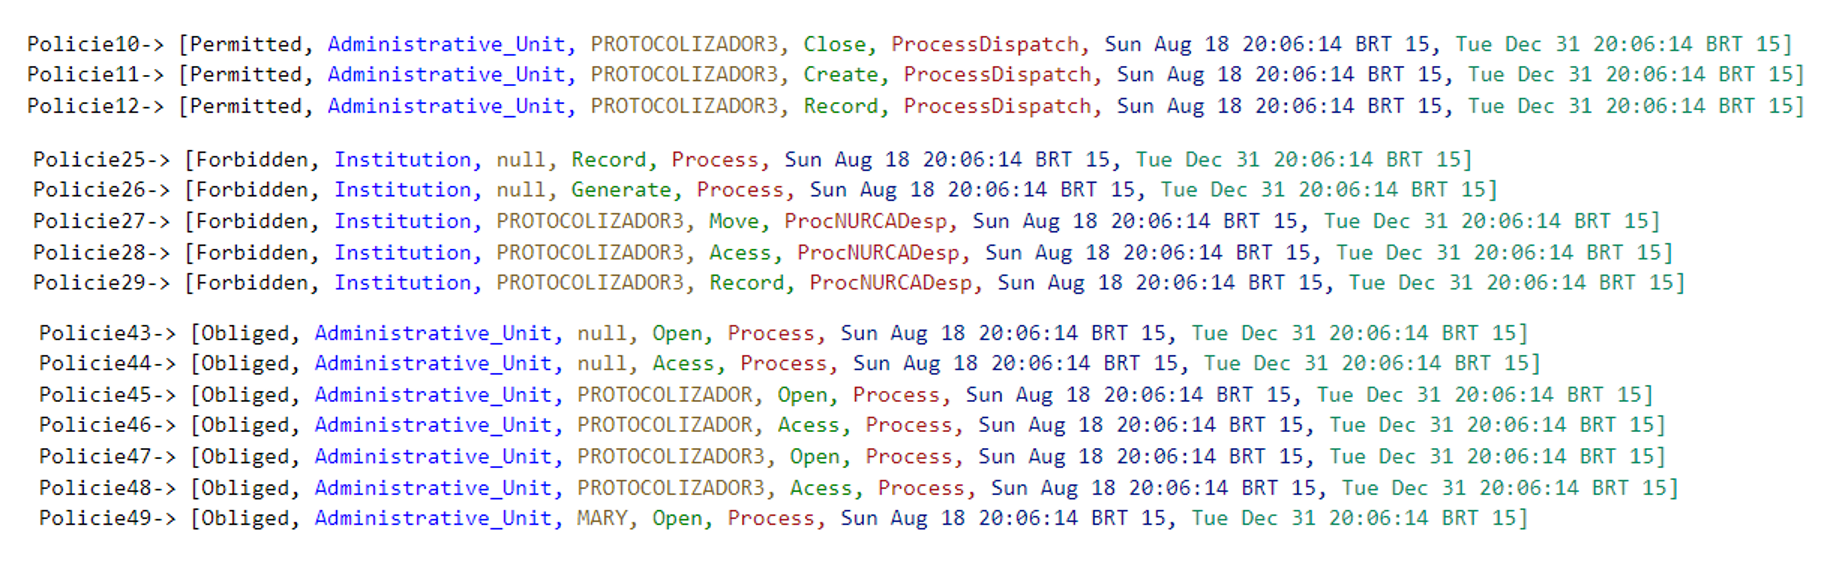
\includegraphics[width=.8\textwidth]{imagens/modelo_politica.png}
	\caption{Modelo das políticas utilizadas no estudo}
	{\scriptsize Fonte: compilação do autor}
	\label{fig:modelo_politica}
\end{figure}

\section{Detecção de conflitos} \label{deteccao_conflitos}

Os conflitos podem ocorrer quando diferentes conjuntos de condições resultam em permitir e negar simultaneamente, ao mesmo papel, à mesma solicitação, ou proibir e obrigar o mesmo papel, à mesma solicitação.

Diz-se que duas regras estão em conflito quando o cumprimento de uma das regras viola a outra e vice-versa. 

Ex:

{\scriptsize \texttt{ \{P1= {\textbf{Permitido}, na Universidade, Paulo, acessar processos administrativos\} }}}

{\scriptsize \texttt{ \{P2= {\textbf{Proibido}, na Universidade, Paulo, acessar processos administrativos\} }}}

A capacidade de um sistema reconhecer um estado inconsistente em andamento ou em potencial é denominada \textbf{detecção de conflitos.}

Em um conflito indireto, as políticas conflitantes regulam ações diferentes (mas relacionadas) executadas por diferentes sujeitos (porém, relacionados) sobre objetos diferentes (mas, relacionados) em organizações diferentes (mas, relacionadas). 

Além disso, um conflito indireto pode ainda ocorrer, mesmo quando as políticas em conflito não têm modalidades contraditórias ou contrárias.

Ex:

{\scriptsize \texttt{P3 = {Obrigado, Empresa E, \textbf{Funcionário, receber}, avaliação, mensal}}}

{\scriptsize \texttt{P4= {Permitido, Empresa E, \textbf{Analista, conceder}, avaliação, mensal}}}

Este conflito não seria detectado diretamente, porém há um conflito se considerarmos os relacionamentos.

\subsection{Trabalhos Relacionados}\label{trabalhos_relacionados}
\cite{bui_efficient_2019} discorre acerca de mineração de dados em políticas de controle de acesso, especificamente do modelo RBAC (\textit{role-based access control}). \cite{lupu_conflicts_1999} discorre sobre conflitos no gerenciamento de sistemas distribuídos com base em políticas de controle de acesso. \cite{koch_conflict_2002}, estudou a detecção e resolução de conflitos nas especificações das políticas de controle de acesso. \cite{neri_conflict_2012}, abordou a detecção de conflitos em políticas de segurança usando a tecnologia da Web Semântica.

\cite{obaidat_multilayer_1994} aborda um sistema de rede neural multicamada para segurança de acesso a computadores. \cite{christodoulou_collision_2008} aborda a detecção de conflitos sobre a ótica da prevenção de colisões no voo livre de aeronaves comerciais usando redes neurais e programação não linear. \cite{mukkamala_intrusion_2002} estuda a detecção de invasões usando redes neurais e máquinas de vetores de suporte. Neste último trabalho a ideia é descobrir padrões úteis ou características que descrevam o comportamento intrusivo de um usuário em um sistema e os autores usam este conjunto de características para construir classificadores que puderam reconhecer anomalias e intrusões conhecidas. 

\cite{jin_development_2002} aborda o desenvolvimento e adaptação de redes neurais probabilísticas construtivas na detecção de incidentes em rodovias. \cite{debar_neural_1992} estuda um componente de rede neural para um sistema de detecção de intrusão. Ainda em detecção de conflitos \cite{chen_flight_2011} trabalha com a detecção e resolução de conflitos de vôo com base em redes neurais.

Todos estes trabalhos foram base para o estudo, amadurecimento bibliográfico e aprofundamento teórico sobre o problema e as soluções propostas neste trabalho, principalmente aqueles relacionados a intrusões e detecção de conflitos aéreos pois não só serviram de inspiração como provavelmente as técnicas possam ser extrapoladas para o uso na detecção de conflitos, tema deste estudo.

Além de \cite{sarkis2017} e \cite{sarkis:artigo:2016} que são os trabalhos- base do estudo da detecção de conflitos, da determinação do modelo das políticas utilizadas e analisadas e das definições utilizadas neste trabalho. Todas as hipóteses e problemas estudados por este trabalho derivam do estudo inicial de \cite{sarkis2017}.

\subsection{Aprendizagem de máquina} \label{aprendizagem_maquina}
Aprendizado de máquina ou \textit{machine learning} é um braço da Inteligência Artificial que emprega técnicas e algoritmos na criação de modelos computacionais dos quais a característica princial é a capacidade de descobrir padrões em um grande volume de dados ou de melhorar o desempenho de uma determinada tarefa através da experiência (do \textit{reforço}).\cite{mohri_foundations_2018} \cite{alpaydin_introduction_2014} \cite{swamynathan_mastering_2019}

Nas palavras de Arthur Lee Samuel, considerado um dos pioneiros na área de inteligência artificial \cite{wiederhold_arthur_1992}, aprendizado de máquina é ``o campo de estudo que dá aos computadores a capacidade de aprender sem serem explicitamente programados". \cite[p. 89]{simon_too_2013}.

Aprendizado de máquina tem sido aplicado na automatização de funções que para os humanos são executadas intuitivamente, mas que são difíceis de definir formalmente. \cite{sarkar_2017}

Assim, de forma geral, a aprendizagem de máquina tem por objetivo estudar e desenvolver métodos computacionais para obter sistemas capazes de adquirir conhecimento de forma automatizada. \cite{lima_ia_2016}

A capacidade de determinados algoritmos tem de aprender a partir de exemplos é chamado de \textbf{aprendizado indutivo}. Estes algoritmos aprendem relacionamentos eventualmente existentes entre os dados, mostrando o resultado nos modelos de conhecimento gerado. \cite{goldschmidt2005}\cite{alpaydin_introduction_2014}

As principais abordagens de aprendizado que determinam os 3 principais tipos de aprendizagem são: a aprendizagem supervisionada, a aprendizagem não-supervisionada e a aprendizagem por reforço. \cite{Norvig2013}. 

Na \textbf{aprendizagem não-supervisionada} o modelo/hipótese busca padrões na entrada, embora não seja fornecido nenhum feedback explícito. Portanto, na abordagem não-supervisionada não há, nos dados, uma classe, não há um rótulo prévio, ou seja, não existe a informação da saída desejada. O processo de aprendizado busca identificar regularidades entre os dados e não é necessária a divisão prévia dos dados em dados de treinamento, validação e teste.  A tarefa mais comum de aprendizagem não supervisionada é o agrupamento. \cite{Norvig2013} \cite{Boscarioli2017} \cite{goldschmidt2005} \cite{aprenda_mineracao_fernando_amaral16}

Na \textbf{aprendizagem supervisionada} o modelo/hipótese observa alguns exemplos de pares de entrada e saída, e aprende uma função que faz o mapeamento entre a entrada e a saída. Portanto, ela compreende a abstração de um modelo a partir dos dados apresentados na forma de pares ordenados (\textit{entrada, saída, saída desejada}). Há, assim, uma \textit{classe}, ou um atributo especial com o qual se pode comparar e validar o resultado.

Na \textbf{aprendizagem por reforço}, aprende-se a partir de uma série de reforços --- recompensas ou punições. Não está disponível, geralmente, na aprendizagem por reforço, para o algoritmo de aprendizado de máquina, um conjunto de dados para treinamento. O aprendizado se dá, então, pela interação com o ambiente que se deseja atuar por um determinado período com o objetivo de melhorar o desempenho de uma determinada tarefa. \cite{Norvig2013} \cite{aprenda_mineracao_fernando_amaral16} \cite{silva_restaurante_2019}	


\subsection{Mineração de Dados}\label{mineracao_dados}
Uma das características de nossa era é produção de dados em grande volume, velocidade e variedade de todas as formas, por dispositivos espalhados em toda parte. Entretanto, dados, mesmo em grande quantidade, são apenas dados. É preciso produzir informação e conhecimento para explorar as vantagens que essa massa pode trazer. O dado necessita ser, de alguma forma, analisado, tratado para que informações e conhecimento possa ser extraído. \cite{aprenda_mineracao_fernando_amaral16} \cite{ferrari2017}

Conforme \cite{fayyad1996}:
\begin{quotation}
	[...] Os computadores permitiram que os humanos coletassem mais dados do que podemos digerir, é natural [,portanto] recorrer a técnicas computacionais para nos ajudar a desenterrar padrões e estruturas significativas a partir dos volumosos volumes de dados. Por isso, [a mineração de dados] é uma tentativa de resolver um problema que a era da informação digital transformou em realidade para todos nós: sobrecarga de dados.
\end{quotation}

Para \cite{Boscarioli2017},
\begin{quotation}
	De forma simplificada, a mineração de dados pode ser definida como um processo automático ou semiautomático de explorar analiticamente grandes bases de dados, com a finalidade de descobrir padrões relevantes que ocorrem nos dados e que sejam importantes para embasar a assimilação de informação importante, suportando a geração de conhecimento. 
\end{quotation}

Ainda, segundo \cite{fayyad1996}, 
\begin{quotation}
	O termo mineração de dados tem sido usado principalmente por estatísticos, analistas de dados e comunidades de sistemas de informações gerenciais (MIS). Ele também ganhou popularidade no campo do banco de dados. O termo descoberta de conhecimento em bancos de dados [(KDD, da sigla em Inglês)] foi cunhada no primeiro workshop do KDD em 1989 para enfatizar que o conhecimento é o produto final de uma descoberta baseada em dados. Foi popularizado nos campos de IA e aprendizado de máquina.
\end{quotation}

Dessa forma, a mineração de dados é parte integrante de um processo mais amplo, conhecido como descoberta de conhecimento em bases de dados (\textit{Knowledge Discovery in Databases}, ou \textit{KDD})\cite{fayyad1996}. Embora se use \textit{mineração de dados} como sinônimo de KDD, a terminologia é empregada para a etapa de \textit{descoberta}  do processo de KDD, que inclui a \textit{seleção} e \textit{integração} das bases de dados, a \textit{limpeza} da base, a \textit{seleção e transformação} dos dados, a \textit{mineração}(propriamente) e a \textit{avaliação} dos dados. \cite{ferrari2017}\cite{Boscarioli2017}.

Assim, a mineração de dados  é definida em termos de esforços para a descoberta de padrões em bases de dados. A partir destes padrões descobertos, há condições de se gerar conhecimento útil para um processo de tomada de decisão (ou a geração de conhecimento para esta tomada).

O KDD (Knowledge Discovery in Database) é um processo de busca de conhecimento em bancos de dados e, de modo geral, consiste de uma sequência iterativa de passos(ou \textbf{etapas})\footnote{O processo de KDD, segundo \cite{fayyad1996} é composto por: \textit{Seleção de dados; Pré-processamento; Transformação; Mineração; Análise e assimilação de resultados}}: limpeza de dados, integração dos dados, Seleção, Transformação e Mineração dos dados, Avaliação dos padrões e Apresentação e Assimilação do conhecimento. Este processo é iterativo e, em alguma etapa, pode-se voltar para uma anterior. \cite{Boscarioli2017}

Neste trabalho as tarefas de seleção e transformação dos dados farão parte da etapa chamada de pré-processamento (cf. \cite{Boscarioli2017} e serão descritas na seção \ref{resultados}.

O termo \textbf{modelo de conhecimento}(ou hipótese) é utilizado na literatura (e neste trabalho) para fazer referência a um padrão ou conjunto de padrões descobertos (que é, enfim, o \textit{propósito} do processo de KDD). Estes padrões são conhecimentos representados segundo as normas sintáticas de alguma linguagem formal. Estes padrões podem ser classificados em dois tipos: preditivos e descritivos. O intuito dos preditivos é resolver um problema específico de prever os resultados ou valores de um ou mais atributos, em função dos valores de outros atributos. Os descritivos (ou informativos) tem o intuito de apresentar informações interessantes e importantes sobre os dados que um especialista de domínio possa não conhecer. Modelos de conhecimento compostos exclusivamente por padrões preditivos são chamados de modelos preditivos, enquanto que modelos descritivos são modelos de conhecimento compostos por padrões descritivos. \cite{goldschmidt2005}\cite{ferrari2017}\cite{Boscarioli2017}

Neste contexto, este trabalho tem como objetivo modelar uma forma de detectar, mediante o uso de técnicas da mineração de dados (e aprendizagem de máquina) os conflitos entre as políticas de controle de acesso de um sistema. Vários algoritmos e técnicas serão utilizados sendo que eles serão devidamente analisados usando-se métricas específicas para cada algoritmo.


\subsection{Algoritmos de classificação}
Conforme \cite{Rocha2012}, ``o termo \textit{classe} deve ser usado quando existe informação sobre quantas e quais são as partições presentes em um conjunto de dados, bem como qual exemplar pertence a qual partição".

Comumente denomina-se \textit{classificação} o processo pelo qual se determina uma função de mapeamento capaz de indicar a qual classe pertence algum exemplar de um domínio sob análise, baseando-se em um conjunto já classificado. \cite{Boscarioli2017}.

Assim, classificação é uma técnica de mineração de dados (aprendizado de máquina) usada para prever a associação ao grupo para instâncias de dados.\cite{classification2013}. É, segundo \cite{aprenda_mineracao_fernando_amaral16} e \cite{performance_classification2013}, a tarefa mais utilizada em mineração de dados. Além de ser a mais complexa e a que possui a maior quantidade de algoritmos disponíveis.\cite{classification2013}	

A classificação é uma das tarefas preditivas de Mineração de Dados e aprendizado de máquina. Tarefas de predição consistem na análise de um dataset (conjunto de dados), descritos por atributos e rótulos associados com o objetivo de descobrir um modelo capaz de mapear corretamente cada um dos dados a seus rótulos. Esse objetivo é alcançado por meio de técnicas chamadas de supervisionadas. A análise preditiva é dividida em categórica, também chamada de classificação ou em numérica, também chamada de regressão. \cite{Boscarioli2017} \cite{classification2013} \cite{ferrari2017} \cite{goldschmidt2005}

Formalmente, a tarefa de classificação pode ser descrita como a busca por uma função de mapeamento para um conjunto $X$ de vetores de entrada (ou, exemplares --- os dados) $\vec{x_i} \in E^d$ para um conjunto finito de rótulos $C$ de cardinalidade $c$. A função $F$ é, então, definida como $F: E^d \times W \rightarrow C$, em que $d$ é a dimensão do espaço $E$, ou seja, a quantidade de coordenadas do vetor $\vec{x_i}$, e $W$ é um espaço de parâmetros ajustáveis por meio do algoritmo de indução supervisionada. \cite{Boscarioli2017}

Pode ser dividida em, ao menos, duas categorias: classificação binária e classificação multiclasse. Na binária, a cardinalidade $c$ é 2. Para o caso em que $c > 2$, o problema é considerado de múltiplas classes.\cite{Boscarioli2017}

Os textos de \cite{classification2013}, \cite{performance_classification2013}, \cite{Wolpert:1996}, \cite{classification_survey2012} e \cite{using_data_mining2012}  trazem reflexões, técnicas, comparações e explicações detalhadas de muitos algoritmos de classificação, entre eles, árvores de decisão, k-vizinhos mais próximos, Naive Bayes e Redes Bayesianas, Redes Neurais Artificiais, Máquinas de Vetores de Suporte (SVM) entre outros.   

Sobre teoria da aprendizagem e algoritmos de classificação há em \cite{Norvig2013} uma discussão sobre qual seria, em relação às hipóteses de modelos de aprendizagem, aquela (ou aquelas) que melhor se ajuste aos dados futuros. O autor cita a \textbf{suposição de estacionaridade}, ou seja, que há uma distribuição de probabilidade sobre os dados que permanece estacionária ao longo do tempo. Supõe-se, portanto que cada exemplo de ponto de dados (antes de conhecê-lo) é uma variável aleatória $E_j$ cujo valor observado $e_j = (x_j, y_j)$ é amostrado da distribuição e é independente dos exemplos anteriores. Assim:
\begin{equation}
P(E_j|E_{j-1},E_{j-2}, ... ) = P(E_j), 
\end{equation}
e cada exemplo tem uma distribuição de probabilidade anterior idêntica:
\begin{equation}
P(E_j) = P(E_{j-1}) = P(E_{j-2}) = ... 
\end{equation}
Estes exemplos são chamados de \textit{independentes e identicamente distribuídos} ou \textbf{i.i.d}. Esta suposição é necessária para tentar a previsão sobre o futuro dos dados. Há claro, ainda em \cite{Norvig2013}, um alerta sobre o fato de ser possível a aprendizagem ocorrer caso haja pequenas alterações (lentas) na distribuição.

Outro fato importante para a definição e avaliação da escolha da melhor hipótese (modelo) de um algoritmo de classificação é definir o ``melhor ajuste". \cite{Norvig2013} define a \textbf{taxa de erro} de uma hipótese como uma métrica importante para definir o ``melhor ajuste" de um modelo/hipótese.

A taxa de erro é, assim, a proporção de erros que o algoritmo classificador comete---a proporção de vezes que $h(x)\neq y$ para o exemplo $(x,y)$ --- sendo $h(x)$ a função que mapeia uma hipótese/modelo $h$ com a previsão/valor conhecido $y$. Nem sempre, como alerta, \cite{Norvig2013}, uma hipótese/modelo(algoritmo) $h$ que tenha uma taxa de erro baixa no conjunto de treinamento generaliza bem. A forma de testar o algoritmo é importante. Para isso há, na literatura, algumas técnicas que são utilizadas como estratégia de treinamento, validação e teste.

Autores como \cite{Boscarioli2017}, \cite{aprenda_mineracao_fernando_amaral16}, \cite{data_science_do_zero2016} e\cite{ferrari2017} citam, como estratégia de treinamento, validação e teste as seguintes técnicas:
\begin{itemize}
	\item Resubstituição;
	\item Holdout;
	\item Validação cruzada;
	\item Bootstrap;
\end{itemize}

Na Resubstituição, segundo \cite{Boscarioli2017}, as medidas de avaliação dos classificadores são aplicadas no próprio conjunto de dados usados para indução do modelo. Essa técnica, embora tenha alguns vantagens discutidas em \cite{ferrari2017} e \cite{Boscarioli2017}, pode levar ao sobreajuste (\textit{overfitting}) discutido em \cite{data_science_do_zero2016}, \cite{aprenda_mineracao_fernando_amaral16} e \cite{Norvig2013}. Basicamente, o sobreajuste é quando se produz um modelo de bom desempenho com os dados de treinamento, mas que não lida bem com novos dados.

Na técnica de \textbf{Holdout}, pressupõem-se uma divisão, ou criação de dois subconjuntos de dados distintos, a partir do conjunto de dados disponível pra uso na indução do modelo/hipótese. Um desses subconjuntos será usado para treinamento (indução) do modelo de previsão e o segundo, para teste após o término do treinamento e, consequentemente, na aplicação das medidas de avaliação do modelo/hipótese.\cite{Boscarioli2017}

A imagem \ref{fig:img_holdout} mostra o funcionamento da técnica de holdout de forma mais detalhada
\begin{figure}[h!]
	\centering
	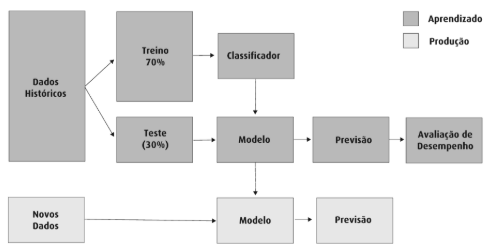
\includegraphics[width=.6\textwidth]{imagens/hold_out.png}
	\caption{Funcionamento da técnica holdout.}
	{\scriptsize Fonte:\cite{aprenda_mineracao_fernando_amaral16}}
	\label{fig:img_holdout}
\end{figure}

Na estratégia de validação cruzada, todos os dados farão parte, em algum momento, do conjunto de dados usado no teste do modelo/hipótese. A ideia é que cada exemplo sirva duplamente --- como dados de treinamento e dados de teste. Primeiro divide-se o conjunto em $k$ subconjuntos iguais. Em seguida realiza-se $k$ rodadas de aprendizagem; em cada iteração $\frac{1}{k}$ dos dados é retido como conjunto de teste e os exemplos restantes são usados como treinamento. Valores populares de $k$ são 5 e 10 --- o suficiente para uma estimativa estatisticamente provável que seja precisa a um custo 5-10 vezes maior no tempo de computação. Há também o extremo do $k = n$, também conhecido como \textbf{validação cruzada com omissão de um}. O método de validação cruzada permite que o modelo/hipótese seja avaliado uma série de vezes, cada série sendo conhecida como partição (ou \textit{fold}). Ao final, a avaliação pode ser realizada aplicando medidas estatísticas como média, desvio-padrão e intervalo de confiança ao conjunto de $k$ avaliações obtidas ou somando-se os desempenhos obtidos pelos $k$ modelos gerados e dividindo essa soma pelo número de exemplares original. \cite{Norvig2013}\cite{Boscarioli2017}\cite{ferrari2017} \cite{aprenda_mineracao_fernando_amaral16}

A imagem \ref{fig:img_cross_validation} mostra um exemplo didático de como funciona a validação cruzada:

\begin{figure}[h!]
	\centering
	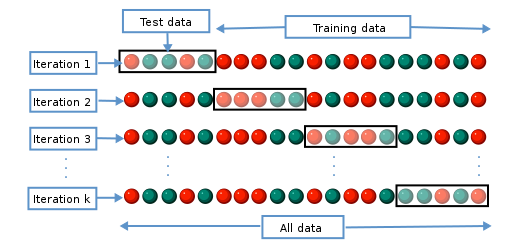
\includegraphics[width=.6\textwidth]{imagens/cross_validation.png}
	\caption{Funcionamento da técnica \textit{cross validation}}
	{\scriptsize Fonte:\cite{fold_cross_validation:k-fold_nodate}}
	\label{fig:img_cross_validation}
\end{figure}

Já a técnica de \textit{Bootstrap} funciona de forma  parecida à estratégia \textit{holdout}. Ela também usa dois conjuntos, um de treinamento e outro para teste, porém durante o processo de formação dos subconjuntos, exemplares que já foram sorteados podem novamente serem contemplados, com probabilidade igual. É uma estratégia que permite, portanto, a reposição.

Neste trabalho, todos os algoritmos de classificação usados foram testados usando as técnicas de resubstituição, \textit{holdout} (com taxas de 70-30 e 60-40), além de \textit{cross-validation} com 3, 5 e 10 folds. Como explicado em \cite{WolpertMacready} e \cite{Wolpert:1996} não existe um algoritmo de aprendizado superior a todos os demais quando considerados todos os problemas de classificação possíveis (teorema \textbf{NFL}, ou \textit{No Free Lunch}), portanto, variações foram executadas nos experimentos em todas técnicas avaliadas, alterando-se os padrões para chegar a métricas e medidas de avaliação mais eficientes.

Há, conforme \cite{Boscarioli2017}, \cite{aprenda_mineracao_fernando_amaral16}, \cite{classification2013} e \cite{classification_survey2012} diversas medidas usadas na avaliação de classificadores. Uma delas (a que será usada neste trabalho) é a acurácia ou taxa de classificações corretas. A acurácia é dada, portanto, por:

\begin{equation}\label{acuracia}
\text{Acurácia} = |y-f(\aleph)=0|,
\end{equation}

em que $|\cdot|$ representa a contagem de vezes em que $\cdot$ é verdadeiro, $f$ é o modelo preditivo, $\aleph$ é o subconjunto de dados sob o qual o modelo está sendo avaliado, $f(\cdot)$ é a classificação fornecida pelo modelo preditivo para cada um dos exemplares (dos dados), e $y$ é a classe esperada como resposta. \cite{Boscarioli2017}

A acurácia de um classificador também pode ser descrita em termos do \textbf{erro de generalização} $\xi_g$, e uma função de perda binária e, portanto, ser interpretada como a probabilidade de ocorrer uma classificação correta. Dessa forma:

\begin{equation}
\text{Acurácia}_g=1 - \xi_g
\end{equation}

Ou seja, a acurácia é, basicamente o número de acertos (positivos) divido pelo número total de exemplos. Será a métrica mais usada para avaliar os classificadores neste trabalho.

\subsection{Redes Neurais artificiais}
As redes neurais instituem um campo da ciência da computação, parte da área da inteligência artificial, que busca efetivar modelos matemáticos que se assemelhem às redes neurais biológicas. Elas apresentam capacidade de adaptar seus parâmetros como resultado da interação com o meio externo. \cite{ferneda_redes_2006}\cite{Norvig2013}

De acordo com \cite[p. 47]{lima_ia_2016}, ``redes neurais podem ser caracterizadas como modelos computacionais com capacidades de adaptar, aprender, generalizar, agrupar ou organizar dados".

Inicialmente, portanto, se desenvolveram como uma estratégia de simular os processos mentais humanos, como reconhecimento de imagens e sons, e após, como instrumento tecnológico e eficienten para muitas tarefas. \cite{jin_development_2002}	

Para \cite{obaidat_multilayer_1994}, as redes neurais artificiais podem ser usadas efetivamente para prover soluções para um amplo espectro de aplicações, incluindo mapeamento de padrões e classificação, análise e codificação de imagens, processamento de sinais, otimização, manipulação de grafos, reconhecimento de caracteres, reconhecimento automático de alvo,  	fusão de dados, processamento de conhecimento, controle de qualidade, mercado de ações, processamento de hipotecas, triagem de créditos para empréstimos entre muitos outros problemas. 

Desde a década de 1940 com o trabalho de \cite{mcculloch_logical_1943} que se busca um modelo computacional que simule o cérebro humano e suas conexões. O interesse pela pesquisa nesta área cresceu e se desenvolveu durante os anos 50 e 60. É dessa época que \cite{rosenblatt_perceptron:_1958} sugeriu um método de aprendizagem para as redes neurais artificiais chamado \textit{percepton}. 

Até o final da década de 1960 muitos trabalhos foram feitos usando o percepton como modelo, mas ao final desta década, \cite{minsky_perceptrons:_1969} apresentaram significativas limitações do perceptron. A pesquisa diminui consideravelmente nos anos seguintes, porém durante  os  anos  80,  a excitação	ressurge mediante os avanços metodológicos importantes e, também, ao aumento dos recursos computacionais disponíveis. O  modelo  de  neurônio  artificial  da figura \ref{fig:neuronio} é uma
simplificação do apresentado por \cite[p. 36]{haykin_redes_2001}

\begin{figure}[h!]
	\centering
	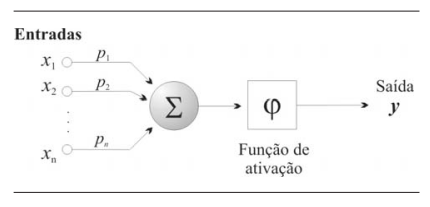
\includegraphics[width=.7\textwidth]{imagens/modelo_matematico_neuronio.png}
	
	{\scriptsize Fonte:\cite[p. 36]{haykin_redes_2001}}
	\caption{Modelo matemático de um neurônio}
	\label{fig:neuronio}
\end{figure}

Este modelo acima (da figura \ref{fig:neuronio}) é composto por três elementos:

\begin{itemize}
	\item  um conjunto de $ n $ conexões de entrada ($ x_1, x_2, ... , x_n $), caracterizadas por pesos ($ p_1, p_2, ..., p_n $);
	\item um somador ($ \sum $) para acumular os sinais de entrada;
	\item uma função de ativação ($\varphi$) que, no caso do neurônio de McCullock-Pitts \cite{mcculloch_logical_1943} é uma função de limiar. \cite{ferneda_redes_2006} \cite{lima_ia_2016}
\end{itemize}

O comportamento das conexões entre os neurônios é simulado através de seus pesos  ($ p_1, p_2, ..., p_n $). Os valores podem ser positivos ou negativos (dependendo se a conexão é inibitiva ou excitativa. O efeito de um sinal proveniente de um neurônio é determinado pela multiplicação do valor do sinal recebido pelo peso da conexão correspondente ($x_i \times p_i$). Então é efetuada a soma dos valores $x_i \times p_i$ de todas as conexões e o valor resultante é enviado para a função de ativação que define a saída ($y$) do neurônio.\cite{Norvig2013}\cite{mcculloch_logical_1943}\cite{minsky_perceptrons:_1969}\cite{ferneda_redes_2006}\cite{haykin_redes_2001}

As redes neurais artificiais (\textbf{RNA}) se formam quando diversos neurônios se combinam. De forma resumida, ``uma rede neural artificial (RNA) pode ser vista como um grafo onde os nós são os neurônios e as ligações fazem a função das sinapses". Isto está demonstrado na figura \ref{fig:rna}

\begin{figure}[h!]
	\centering
	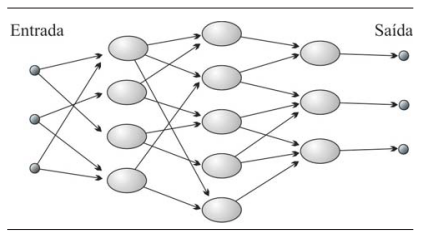
\includegraphics[width=.7\textwidth]{imagens/RNA.png}	
	\caption{Representação simplificada de uma RNA}
	{\scriptsize 	Fonte: \cite[p.26]{ferneda_redes_2006}}
	\label{fig:rna}
\end{figure}

As  redes  neurais  artificiais  se  diferem  pelas  suas arquiteturas e pela forma como os pesos associados às conexões são ajustados durante o processo de aprendizado.	A arquitetura de uma rede neural restringe o tipo de problema no qual a rede poderá ser utilizada, e é definida pelo  número  de  camadas  (camada única  ou múltiplas camadas), pelo número de nós em cada camada, pelo tipo de conexão entre os nós (\textit{feedforward} ou \textit{feedback}) e por sua topologia. \cite[p. 46-49]{haykin_redes_2001}

O desenvolvimento de uma rede neural artificial consiste em determinar sua arquitetura, ou seja, os números de camadas e de neurônios em cada camada, bem como o ajuste dos pesos na fase conhecida como treinamento.\cite{hagan_neural_1996} \cite{haykin_redes_2001}

Uma das características mais importantes de uma rede neural artificial é a habilidade de aprender através de exemplos e fazer inferências sobre o que aprendeu, melhorando, assim, o seu desempenho. As RNA's utilizam um algoritmo de aprendizagem que serve, basicamente, para ajustar os pesos de suas conexões. \cite{haykin_redes_2001} \cite{ferneda_redes_2006} \cite{lima_ia_2016} \cite{Norvig2013}. Aqui também há, cf. explicitado na seção \ref{aprendizagem_maquina}, duas formas básicas de aprendizado, o supervisionado e o não-supervisionado.

\subsection{SVM - Support Vector Machines}\label{SVM}
Segundo \cite{cortes_svm_1995}, o algoritmo SVM (\textit{Support Vector Machines}) é um dos mais efetivos para a tarefa de classificação.

Cf. \cite{goldschmidt2005},
\begin{quotation}
	No algoritmo SVM, o conjunto de dados de entrada é utilizado para construir uma \textit{função de decisão} $f(x)$, tal que:
	
	\begin{table}[h!]
		\centering
		\begin{tabular}{lll}			
			$ Se \ f(x_i) \geq 0,  $ & então   & $ y_i = 1 $  \\
			$ Se \ f(x_i) < 0, $ & então & $ y_i = -1 $  
		\end{tabular}
	\end{table}
	
	O algoritmo SVM constrói os denominados classificadores lineares, que separam o conjunto de dados por meio de um hiperplano que é a generalização do conceito de \textit{plano} para dimensões maiores que três.	
\end{quotation}

Assim, SVM, cf. \cite[p. 45]{aprenda_mineracao_fernando_amaral16} ``são um algoritmo de classificação que maximizam as margens entre instâncias mais próximas, dessa forma, é criado um vetor otimizado que é então utilizado para classificar novas instâncias".

Conforme se vê na figura \ref{fig:svm}, os dois vetores \textit{não pontilhados} são as margens otimizadas. As instâncias por onde as margens otimizadas passam são os vetores de suporte. O vetor pontilhado é a referência para classificar novas instâncias. Assim, a nova instância, na figura \ref{fig:svm} é classificada como triângulo.

\begin{figure}[h!]
	\centering
	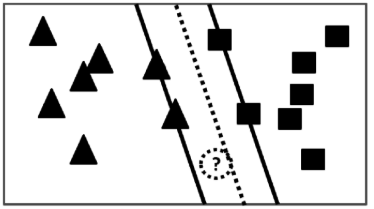
\includegraphics[width=.7\textwidth]{imagens/vetores_de_suporte.png}	
	\caption{Vetores de Suporte}
	\label{fig:svm}
	{\scriptsize 	Fonte: \cite[p. 45]{aprenda_mineracao_fernando_amaral16}}
\end{figure}

Seguindo o estudo de \cite{mukkamala_intrusion_2002} há duas razões principais que levaram os autores do artigo citado de usarem SVMs para detecção de intrusão:o primeiro é a velocidade já que a performance é prioritariamente uma das características mais importantes para sistemas de detecção de intrusos. A segunda razão é a escalabilidade, pois, cf. os autores, SVMs são relativamente indiferentes ao número de \textit{data points} e a complexidade da classificação não depende da dimensionalidade do espaço de características. Dependendo da aplicação, ainda conforme os autores, uma vez que os dados estão classificados em duas classes, um algoritmo de otimização adequado pode ser usado, se necessário,  para identificação de mais características.

Neste trabalho, também foi usado, com boa eficácia (cf. se vê na seção \ref{resultados}) o algoritmo SVM.

\chapter{Experimentos/Resultados}\label{resultados}
Para os experimentos, um arquivo de políticas foi gerado a partir do proposto em \cite{sarkis2017} e, de acordo com o exposto na seção \ref{modelo_politica_utilizada}. O arquivo gerado possui cerca de 68 políticas nomeadas (constituindo a \textit{fase de seleção}\footnote{cf. seção \ref{mineracao_dados} deste trabalho.} da Mineração de Dados). 

Este arquivo foi usado nos testes preliminares da hipótese:  \textit{Converter a detecção de conflitos a um problema de classificação reestruturando os atributos} (colunas). Para este problema da detecção de conflitos diretos serão usadas técnicas de aprendizagem supervisionada. Para tanto, ao arquivo com as políticas, no pré-processamento foi acrescentada uma coluna rotulando os conflitos da seguinte forma: \textbf{1}: \textit{conflito direto} e \textbf{0}: \textit{sem conflito}.

A figura \ref{fig:aspecto_arquivo} demonstra o aspecto do arquivo das políticas geradas paraos experimentos deste trabalho. Na imagem, pode-se notar a classe (coluna) criada para guiar o aprendizado supervisionado dos algoritmos utilizados no estudo.

\begin{figure}[h!]
	\centering
	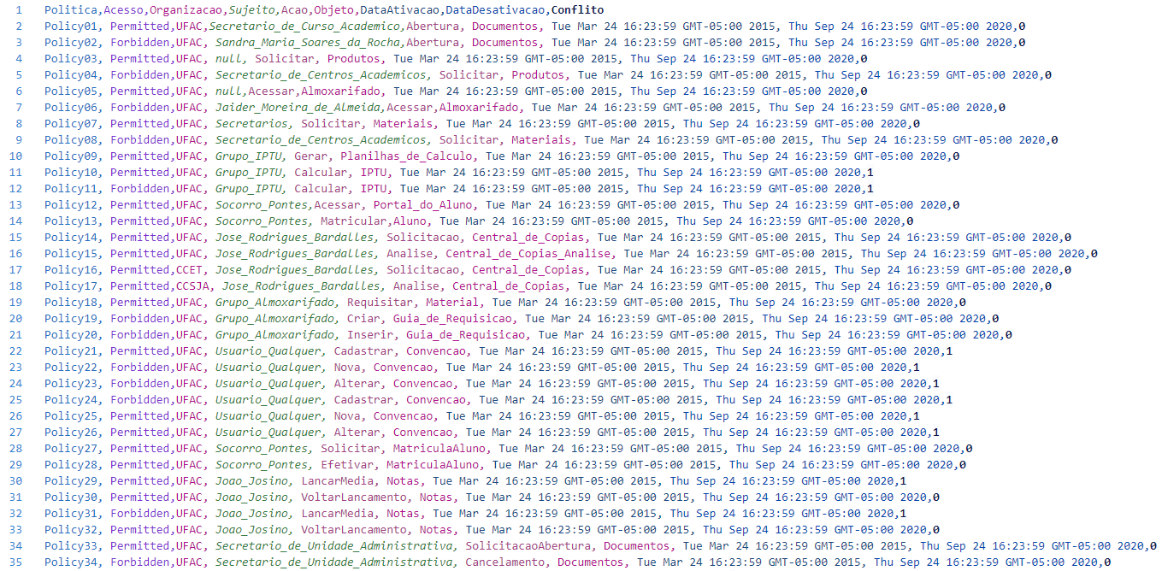
\includegraphics[width=.8\textwidth]{imagens/aspecto_arquivo_politicas.png}	
	\caption{Aspecto do arquivo das políticas geradas para os experimentos}
	\label{fig:aspecto_arquivo}
	{\scriptsize Fonte: compilação do autor}
\end{figure}

Dois \textbf{ambientes computacionais} foram utilizados para as tarefas de mineração: 
um \textbf{notebook}  Intel Core i5 vPro-8350U (8ª Geração de 64 bits com 1.70GHz e 8 GB de RAM, com SSD de 256 GB rodando Windows 10 Pro. 
O outro ambiente foi um \textbf{Desktop} Intel Core i7 vPro-6700 de 8ª geração de 64 bits com 3.40 Ghz e 20 GB de RAM, com HD de 1 TB rodando o Windows 10 Pro.

Ainda na fase de \textit{pré-processamento}, a coluna 9 (Conflito) foi transformada do tipo de dado \textit{Numérico para Nominal}. Para isso foi usada o softwate WEKA (descrito em \cite{eibe2016}) aplicado o filtro \textit{NumericToNominal} do software.

Logo após, mais de 30 experimentos foram realizados de forma preliminar no \textit{dataset} envolvendo os diversos algoritmos e muitos parâmetros alterados (a maioria com pequena ou nenhuma variação) para se chegar às técnicas finais que foram utilizadas nos posteriores experimentos e que serão explicitadas a seguir.

Utilizando-se a ferramenta WEKA (\cite{eibe2016}) para as últimas fases do KDD (Mineração de Dados), foram utilizados alguns algoritmos de classificação que segundo \cite{wu2007} são alguns dos mais utilizados na Mineração de Dados. Para avaliar o desempenho definiu-se o método cross-validation com 10 folds. Em seguida suas acurácias foram comparadas.

A tabela \ref{tab:acuracias} mostra o resultado destes experimentos:

\begin{table}[h!]
	\centering
	\caption{Acurácia dos classificadores}
	\label{tab:acuracias}
	\vspace{0.3cm}
	\begin{tabular}{p{6cm}c}
		\hline\\
		Classificador/Algoritmo& Acurácia  \\[10pt] 
		\hline
		Multi Layer Perceptron & 0.9705    \\
		Random Forest~         & 0.9558    \\
		J48                    & 0.9411    \\
		K* (K-star)            & 0.9411    \\
		Trees LMT              & 0.9117    \\
		IBk (KNN, com k =1)~   & 0.8970    \\
		JRip                   & 0.8970    \\
		SVM kernel linear~     & 0.8676    \\
		Nayve Bayes            & 0.8674    \\
		Random Tree            & 0.7794    \\
		\hline
	\end{tabular}
	\\[6pt]	\centering {\footnotesize Fonte: Elaborada pelo autor mediante experimentos}	
\end{table}

As figuras \ref{fig:saida_svm} e \ref{fig:saida_multilayerperceptron} mostram os resultados das classificações do arquivo de políticas usando, respectivamente, os classificadores/algoritmos: \textit{SVM} e o \textit{MultiLayer Perceptron} (que foram os principais citados nos trabalhos relacionados, cf. descrito na seção \ref{trabalhos_relacionados}). Importante ressaltar que outros classificadores, como o Random Forest, o J48, o K* e o KNN tiveram resultados superiores (em termos de acurácia e precisão) ao SVM, cf. mostrado na tabela \ref{tab:acuracias}. Entretanto, no referncial teórico, o SVM foi citado diversas vezes na detecção de alguns tipos de conflitos e em outras tarefas de classificação de diversos conjuntos de dados.
\begin{figure}[h!]
	\centering
	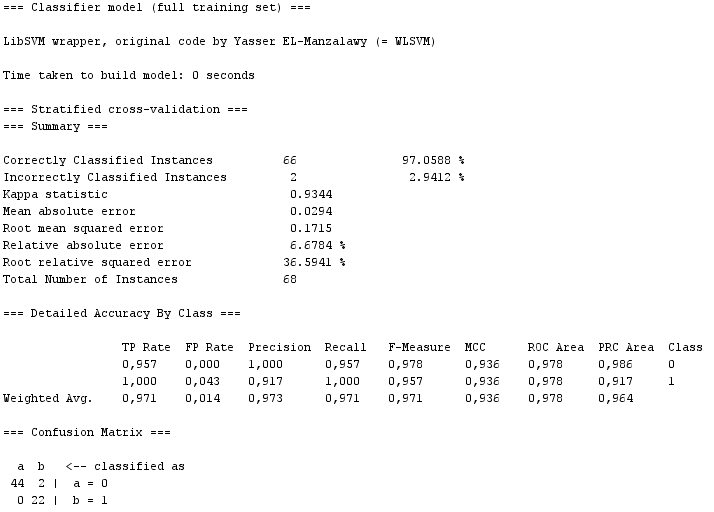
\includegraphics[width=.7\textwidth]{imagens/svm-resultados.png}	
	\caption{Saída do software WEKA. Classificador: SVM}
	\label{fig:saida_svm}
	{\scriptsize Fonte: compilação do autor}
\end{figure}
\begin{figure}[h!]
	\centering
	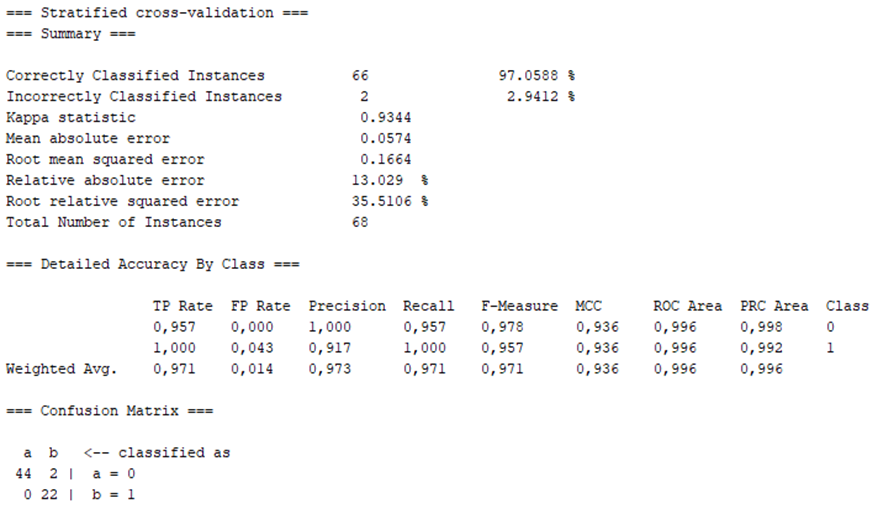
\includegraphics[width=.7\textwidth]{imagens/multilayerperceptron-resultados.png}
	\caption{Saída do software WEKA. Classificador: \textit{MultiLayer Perceptron}}
	\label{fig:saida_multilayerperceptron}
	{\scriptsize Fonte: compilação do autor}
\end{figure}

Assim, com uma acurácia de 97,05\% na classificação dos conflitos diretos, o algoritmo Multilayer Perceptron (que implementa uma rede neural sigmoide multicamadas) foi o que teve a maior acurácia, com 95,7\% de \textit{TP rate}(taxa de \textit{True Positives} ou verdadeiros positivos) para a classe 0 (não há conflito) e, somente, 4,3\% de \textit{FP rate}(taxa de Falsos Positivos) para a classe 1 (quando há conflito direto). Nos experimentos realizados (assim como se esperava inicialmente na hipótese deste trabalho --- baseado em evidências da literatura), este modelo algorítmico foi o mais eficiente para a detecção de conflitos diretos.

\chapter{Propostas para a dissertação}\label{propostas}
Para a pesquisa que resultará na dissertação de mestrado os seguintes pontos serão levantados, estudados e melhor definidos em termos dos objetivos do trabalho:
\begin{itemize}
	\item Pesquisar sobre o relacionamento entre entidades, ações e definições sobre políticas (para entendimento da propagação de políticas);
	\item Construção (teoria) e Programação (prática) do Perceptron (com \textit{backpropagation} para ajuste de pesos e atributos --- treinamento da rede neural);
	\item Análise da função de ativação no classificador;
	\item Análise teórica e construção da Função soma (e funções sigmóides de ativação do perceptron);
	\item Análise teórica e construção das múltiplas layers do perceptron;
	\item Usar Reinforcement Learning e Deep Learning para a detecção dos conflitos indiretos;
	\item Comparação com outros classificadores (preferencialmente, geométricos, como o KNN e o SVM, avaliando suas acurácias e eficiência.
\end{itemize}

\chapter{Conclusões}\label{conclusoes}
\begin{itemize}
	\item Esta pesquisa mostrou que é possível \textit{converter a detecção de conflitos a um problema de classificação} conforme demonstrado neste trabalho, especificamente, para os conflitos \textbf{\textit{diretos}};
	\item O classificador mais acurado, nos experimentos, foi, como se imaginava pela hipótese, o \textit{MultiLayer Perceptron} que é um classificador que usa \textit{backpropagation} para aprender usando perceptron de várias camadas para classificar instâncias desconhecidas \cite{eibe2016};
	\item Este será um dos classificadores usados para detectar conflitos indiretos. O outro será o SVM (e outros classificadores geométricos). Suas acurácias serão devidamente comparadas juntamente com a eficiência das soluções propostas.
\end{itemize}